\documentclass[10pt, xcolor=x11names, compress]{beamer}
\usetheme{progressbar}
\progressbaroptions{headline=sections,titlepage=normal,frametitle=normal}
\setbeamertemplate{navigation symbols}{}
\usepackage{iwona}

\usepackage{alltt}
\usepackage{amsmath,amsfonts, amssymb, amscd}
\usepackage{hyperref}
\usepackage{setspace}

\usepackage[overlay,absolute]{textpos}
\TPGrid[5mm,5mm]{20}{20}

\renewcommand{\Re}{\operatorname{Re}}
\renewcommand{\Im}{\operatorname{Im}}

\newcommand{\chik}{$\chi(k)$}
\newcommand{\chir}{$|\tilde{\chi}(R)|$}


\newcommand{\file}[1]{{\color{Firebrick4}\texttt{`#1'}}}

\mode<presentation>

\definecolor{ExampleGreen}{rgb}{0,0.6,0} 


\title{The XAFS Experiment}

\subtitle[]{Instrumentation, Sample Preparation, and Experiment
  Design}

\author[Bruce Ravel]{Bruce Ravel}
\institute[NIST]{
  Synchrotron Methods Group, Ceramics Division\\%
  Materials Measurement Laboratory\\%
  National Institute of Standards and Technology\\%
  \&\\%
  Local Contact, Beamline X23A2\\%
  National Synchrotron Light Source\\[3ex]~}

\date[1$^{\mathrm{st}}$ ASEAN XAS]{1$^{\mathrm{st}}$ ASEAN Workshop on
  X-ray Absorption Spectroscopy\\Synchrotron Light Research
  Institute\\Nakhon Ratchasima, Thailand \\29--31 July 2010}

%\logo{\includegraphics[width=1.0cm]{images/ankaxas_black.jpg}}


\begin{document}
\begin{frame}
  \titlepage
\end{frame}
%
\begin{frame}
  \frametitle{Copyright}
  \tiny

  This document is copyright \copyright\ 2010-2015 Bruce Ravel.

  \begin{center}
    \includegraphics[width=1.0cm]{cc-by-sa.png}
  \end{center}

  This work is licensed under the Creative Commons
  Attribution-ShareAlike License.  To view a copy of this license,
  visit \href{http://creativecommons.org/licenses/by-sa/3.0/}
  {\color{Purple4}\texttt{http://creativecommons.org/licenses/by-sa/3.0/}}
  or send a letter to Creative Commons, 559 Nathan Abbott Way,
  Stanford, California 94305, USA.

  \begin{description}[Under the following conditions:]
  \tiny
  \item[You are free:] %
    \begin{itemize}
      \tiny
    \item \textbf{to Share} --- to copy, distribute, and transmit the work
    \item \textbf{to Remix} --- to adapt the work
    \item to make commercial use of the work
    \end{itemize}
  \item[Under the following conditions:] %
    \begin{itemize}
      \tiny
    \item \textbf{Attribution} -- You must attribute the work in the manner
      specified by the author or licensor (but not in any way that
      suggests that they endorse you or your use of the work).
    \item \textbf{Share Alike} -- If you alter, transform, or build upon this
      work, you may distribute the resulting work only under the same,
      similar or a compatible license.
    \end{itemize}
  \item[With the understanidng that:] 
    \begin{itemize}
      \tiny
    \item \textbf{Waiver} -- Any of the above conditions can be waived
      if you get permission from the copyright holder.
    \item \textbf{Public Domain} -- Where the work or any of its
      elements is in the public domain under applicable law, that
      status is in no way affected by the license.
    \item \textbf{Other Rights} -- In no way are any of the following
      rights affected by the license:
      \begin{itemize}
      \tiny
      \item Your fair dealing or fair use rights, or other
        applicable copyright exceptions and limitations;
      \item The author's moral rights;
      \item Rights other persons may have either in the work itself
        or in how the work is used, such as publicity or privacy
        rights.
      \end{itemize}
    \item \textbf{Notice} -- For any reuse or distribution, you must
      make clear to others the license terms of this work.
    \end{itemize}
  \end{description}

  This is a human-readable summary of the Legal Code (the full
  license).


\end{frame}

%%% Local Variables:
%%% mode: latex
%%% End:




%% \section*{Outline}
%% \begin{frame}
%%   \tableofcontents
%% \end{frame}

\section{The synchrotron}
\label{sec:synch}

\subsection{The facility}

\begin{frame}
  \frametitle{The floor of the synchrotron}
  
  \begin{center}
    \includegraphics[width=0.8\linewidth]{synch/SOL008h.jpg}
    
    \smallskip

    All synchrotron facilities have the same basic layout consisting
    of a storage ring with radiation emitted radially into beamlines.
    Beamlines consist of optics to condition the beam for experiments.
  \end{center}
  \begin{textblock*}{0.5\linewidth}(0pt,20\TPVertModule)%
    \tiny%
    Drawing courtesy of Synchrotron Soleil.
  \end{textblock*}
\end{frame}

\begin{frame}
  \frametitle{Why build synchrotrons?}
  \begin{columns}
    \begin{column}{0.55\linewidth}
      \begin{center}
        \includegraphics[width=0.9\linewidth]{synch/brilliance.png}
      \end{center}
    \end{column}
    \begin{column}{0.45\linewidth}
      Photon properties produced by a synchrotron:
      \begin{itemize}
      \item High flux
      \item Small source size
      \item Broad range of energies (wavelengths)
      \item Extremely collimated
      \item Time structure
      \item Polarized
      \end{itemize}
    \end{column}
  \end{columns}
  \begin{block}{Brilliance}
    A metric that positively quantifies more flux, less divergence,
    and smaller source size.
  \end{block}
\end{frame}

\begin{frame}
  \frametitle{The storage ring}
  \begin{columns}
    \begin{column}{0.55\linewidth}
      \begin{center}
        \includegraphics[width=0.9\linewidth]{synch/SLSstorage.jpg}
      \end{center}
    \end{column}
    \begin{column}{0.45\linewidth}
      \begin{center}
        \includegraphics[width=0.9\linewidth]{synch/storage.png}
      \end{center}
    \end{column}
  \end{columns}

  \medskip

  The storage ring is a large, evacuated, \alert{polygonal}
  tube for containing relativistic electrons.  Along with various
  kinds of magnets used to condition and shape the stored current, the
  ring has special magnets which generate useful X-rays as the
  electrons pass through.

  \begin{enumerate}
  \item Bending magnets
  \item Insertions devices: wigglers and undulators
  \end{enumerate}

  \begin{textblock*}{0.7\linewidth}(0pt,20\TPVertModule)%
    \tiny%
    Photo courtesy of the Swiss Light Source and drawing courtesy of
    DESY.
  \end{textblock*}
\end{frame}

\subsection{Sources}

\begin{frame}
  \frametitle{Bend magnets}
  \framesubtitle{Overview}
  \begin{columns}
    \begin{column}{0.65\linewidth}
      \begin{center}
        \includegraphics[width=0.7\linewidth]{synch/ALSbend.jpg}
      \end{center}
      
      \small

      Bend magnets serve two purposes:
      \begin{itemize}
      \item Steer the electrons between straight sections
      \item Generate photons for use in a beamline
      \end{itemize}
      With relativistic electrons, the light emitted by
      the bend magnet is in a narrow cone.

    \end{column}
    \begin{column}{0.35\linewidth}
      \begin{center}
        \includegraphics[width=0.9\linewidth]{synch/bend.png}
      \end{center}
    \end{column}
  \end{columns}
  \begin{textblock*}{0.7\linewidth}(0pt,20\TPVertModule)%
    \tiny%
    Photo and drawing courtesy of the Advanced Light Source
    and \href{http://lightsources.org}%
    {\color{Brown4}\texttt{http://lightsources.org}}
  \end{textblock*}
\end{frame}

\begin{frame}
  \frametitle{Bend magnet radiation}
  \framesubtitle{Spectrum}
  \begin{columns}
    \begin{column}{0.5\linewidth}
      \includegraphics[width=\linewidth]{synch/bm.jpeg}
    \end{column}
    \begin{column}{0.5\linewidth}
      BM radiation has a characteristic energy $\varepsilon_c$, the
      \textit{critical energy}, above which half of the total power is
      radiated:
      \begin{center}
        \alert{$\varepsilon_c = 0.665 B_0 E^2$}
      \end{center}
      \begin{itemize}
      \item $B_0$ is the bend magnet field strength
      \item $E$ is the energy of the storage ring
      \end{itemize}
    \end{column}
  \end{columns}

  \smallskip

  \begin{itemize}
  \item All bend magnets excel at delivering photons from the IR through
    the VUV and into the X-ray
  \item Bend magnets at high energy facilities (APS, ESRF, SPring-8)
    deliver useful flux beyond 100 keV.
  \item High energy performance be be tuned by increasing field
    strength, e.g. ALS or SLS \alert{superbend} devices.
  \end{itemize}


  \begin{textblock*}{0.5\linewidth}(0pt,20\TPVertModule)%
    \tiny%
    Drawing courtesy of the ESRF BM25.
  \end{textblock*}
\end{frame}

\begin{frame}
  \frametitle{Insertion devices}

  Insertion devices periodic magnetic structures designed to improve
  upon the performance of bending magnets.

  \smallskip

  They are \alert{inserted into} the straight sections of the storage
  ring.

  \smallskip

  Insertion devices in use around the world range from the enormous
  (APS undulator A, $>2$\,m, on the left) to the compact (the NSLS X25
  minigap undulator, $<1$\,m, on the right).

  \begin{columns}
    \begin{column}{0.5\linewidth}
      \begin{center}
        \includegraphics[width=0.7\linewidth]{synch/APSundulatorA.jpg}
      \end{center}
    \end{column}
    \begin{column}{0.5\linewidth}
      \begin{center}
        \includegraphics[width=0.7\linewidth]{synch/x25mgu.jpg}
      \end{center}
    \end{column}
  \end{columns}
  \begin{textblock*}{0.5\linewidth}(0pt,20\TPVertModule)%
    \tiny%
    Photos courtesy of the APS and NSLS.
  \end{textblock*}
\end{frame}


\begin{frame}
  \frametitle{Wigglers and Undulators}
  \begin{columns}
    \begin{column}{0.4\linewidth}
      \begin{center}
        \includegraphics[width=\linewidth]{synch/id.jpg}\\
        \includegraphics[width=0.7\linewidth]{synch/bm_id.png}
      \end{center}
    \end{column}
    \begin{column}{0.6\linewidth}
      \begin{description}[Wig]
        \footnotesize
      \item[Wiggler] ~\\
        \begin{itemize}
          \footnotesize
        \item A wiggler is, in a sense, a sequence of high field
          dipole magnets.  It is an improvement over a bend magnet
          through a multiplicative effect.
        \item The broadband wiggler spectrum is very similar to
          the BM spectrum, although with much higher flux.
        \item The price a wiggler beamline pays is managing higher
          heat loads.
        \end{itemize}
      \item[Undulator] ~\\
        \footnotesize
        Undulators are similar to wigglers, but the magnet period
        is shorter and the gap is often smaller.  The light from each
        dipole is coherent, resulting in constructive interference and
        greatly enhanced flux at special wavelengths.
      \end{description}
      
      \begin{block}{Undulator XAS beamlines}
        \footnotesize
        XAS requires that the gap and the monochromator be scanned in a
        coordinated manner.
      \end{block}
    \end{column}
  \end{columns}

  \begin{textblock*}{0.5\linewidth}(0pt,20\TPVertModule)%
    \tiny%
    Drawing courtesy of the APS, plot courtesy of DESY.
  \end{textblock*}
\end{frame}


\section{The beamline}
\label{sec:bl}

\begin{frame}
  \frametitle{A typical XAS beamline}
  
  \small
  \begin{center}
    \includegraphics[width=0.7\linewidth]{bl/xas_beamline.png}
  \end{center} 
  \begin{description}[Collimating mirror]
  \item[Source] Behind the shield wall, part of the ring
  \item[Collimating mirror] Removes the vertical divergence of the
    source, making the instrumental energy resolution independent of
    beam size
  \item[Monochromator] Select a single wavelength from the white light
  \item[Focusing mirror] Focus the beam into a small spot
  \item[Endstation] Enclosed space for the sample positioners,
    detectors, and other equipment
  \end{description}
\end{frame}

\subsection{Mirrors}
\begin{frame}
  \frametitle{Collimating and Focusing Mirrors}
  \begin{block}{Total external reflection}
    A mirror is smooth ({\AA}ngstrom roughness) Si, SiO$_2$ or other
    material, often coated with a metal (Ni, Pt, Rh).
  \end{block}

    \medskip

  \begin{center}
    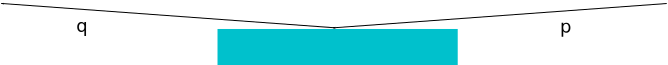
\includegraphics[width=0.7\linewidth]{bl/reflection.png}

    \medskip

    \begin{tabular}[h]{lcl}
      \multicolumn{3}{l}{\alert{Focusing}}\\[1ex]
      Parabolic curvature $\parallel$ beam & $R_m = \frac{2pq}{(p+q)\sin\theta}$ & typically km \\[1ex]
      Cylindrical curvature $\perp$ to beam & $R_s = \frac{2pq\sin\theta}{p+q} $  & typically cm \\[1ex]
      (De)Magnification & $M = \frac{q}{p}$ & ~ \\[4ex]
      \multicolumn{3}{l}{\alert{Collimation}}\\[1ex]
      $q\rightarrow\infty$ & $R_m = \frac{2p}{\sin\theta} $ & ~ \\[1ex]
      Collimation limited by source size & $\delta\theta = S_v/p$ & ~
    \end{tabular}
  \end{center} 
\end{frame}

\begin{frame}
  \frametitle{Mirrors}
  \begin{columns}
    \begin{column}{0.5\linewidth}
      \begin{center}
        \includegraphics[width=0.7\linewidth]{bl/Toroidal.jpg}
      \end{center} 
    \end{column}
    \begin{column}{0.5\linewidth}
      A toroidal focusing mirror is polished into a cylinder and
      mounted on a meridional bender.

      \smallskip

      The full apparatus is placed in a vacuum vessel and mounted on a
      vibration isolating support.
      \begin{center}
        \includegraphics[width=\linewidth]{bl/mirrortank.jpg}
      \end{center} 
    \end{column}
  \end{columns}
  \begin{textblock*}{0.5\linewidth}(0pt,20\TPVertModule)%
    \tiny%
    Photos courtesy of ESRF and Bruker EST
  \end{textblock*}
\end{frame}

\subsection{Mono}
\begin{frame}
  \frametitle{Monochromator : overview}
  \begin{columns}
    \begin{column}{0.6\linewidth}
      The mono is the device that turns white light (all energies)
      into monochromatic light (single energy).
    \end{column}
    \begin{column}{0.4\linewidth}
      \includegraphics[width=\linewidth]{bl/mono.pdf}  
    \end{column}
  \end{columns}
  \begin{columns}
    \begin{column}{0.5\linewidth}
      \begin{center}
        \includegraphics[width=0.8\linewidth]{bl/mono_interior.jpg}
      \end{center}
    \end{column}
    \begin{column}{0.5\linewidth}
      \begin{center}
        \includegraphics[width=0.8\linewidth]{bl/mono_exterior.jpeg}
      \end{center}
    \end{column}
  \end{columns}
\end{frame}

\begin{frame}
  \frametitle{Monochromator : Bragg diffraction}

  \begin{itemize}
  \item The mono uses a very pure crystal to select specific energies
    (wavelengths) by Bragg diffraction.
  \item The crystal diffracts according to Bragg's law:
    \begin{center}
      \begin{columns}
        \begin{column}{0.45\linewidth}
          \includegraphics[width=\linewidth]{bl/bragg.png}
        \end{column}
        \begin{column}{0.2\linewidth}
          \Large
          $\lambda = \frac{2\pi\hbar c}{E}$
        \end{column}
      \end{columns}
    \end{center}
    At a specific angle $\theta$, photons of a specific energy
    (equivalently, a specific wavelength $\lambda$) meet the Bragg
    condition.
  \item The \alert{first crystal} directs the beam towards the
    ceiling!
  \item The \alert{second crystal} steers the beam in the same
    direction as the incident beam, but displaced vertically.
  \item Common crystals: Si(111), Si(220), Si(311), InSb, beryl,
    diamond, YB$_{66}$
  \end{itemize}

\end{frame}


\begin{frame}
  \frametitle{Harmonics}
  \begin{alertblock}{Caution: Harmonic content of beam}
    $2d\sin(\theta) = \alert{n}\lambda$ \qquad
    Higher energies with wavelength $\frac1n$ of the fundamental also
    satisfy the Bragg condition!  Something must be done to remove
    harmonics from the beam.
  \end{alertblock}
  \begin{columns}
    \begin{column}{0.5\linewidth}
      \begin{center}
        Harmonic rejection mirror

        \includegraphics[width=0.9\linewidth]{bl/mir.png}

      \end{center}
      \footnotesize
      The critical angle of any mirror is energy dependent.
    \end{column}
    \begin{column}{0.5\linewidth}
      \begin{center}
        2$^{nd}$ Crystal detuning

        \includegraphics[width=0.9\linewidth]{bl/detune.png}
      \end{center}

      \footnotesize
      The rocking curve of the harmonic is much narrower than the
      fundamental. 
    \end{column}
  \end{columns}
\end{frame}

\section{The sample}
\label{sec:sample}

\begin{frame}
  \frametitle{Sample preparation}
  
  \begin{exampleblock}{The basic rule of sample preparation}
    Ideally, the sample is homogeneous so that every ray of light
    interacts identically with every part of the sample.
  \end{exampleblock}

  To the extent that you are capable of doing so, you should always
  prepare your sample with this in mind.

  \bigskip

  Really good samples include things like:
  \begin{itemize}
  \item Solutions and suspensions
  \item Fine powders dispersed in a binder like BN, graphite, or
    cellulose
  \item Uniform films
  \item Adsorbed species in uniformly dispersed biomass
  \item \quad... and so on ...
  \end{itemize}
\end{frame}

\subsection{Transmission}

\begin{frame}
  \frametitle{Absorption depth}
  
  I recently needed to prepare powders of LaTiO$_2$N for
  transmission XAS at the Ti K edge.

  \smallskip

  \begin{columns}
    \begin{column}{0.6\linewidth}
      \includegraphics[width=0.9\linewidth]{sample/heph_formula.png}
    \end{column}
    \begin{column}{0.4\linewidth}
      Using \textsc{hephaestus}, I computed the absorption depth of
      LaTiO$_2$N at 5\,keV (just above the Ti K edge).

      \medskip

      The answer is \alert{5.2 microns}!
    \end{column}
  \end{columns}

  \begin{alertblock}{What is the consequence of such a short
      absorption length?}
    Answer: For transmission, you need {\tiny small} particles.
  \end{alertblock}
\end{frame}

\begin{frame}
  \frametitle{The problem with large particles}
  \begin{columns}
    \begin{column}{0.6\linewidth}
      If your particles are large compared to an absorption length,
      then your sample will look something like this:

      \bigskip

      \begin{alertblock}{This is bad!}
        Some regions are very thick, while other regions have gaps (or
        leakage).  The leakage problem distorts the your data by
        decreasing white line height and altering the measured
        $\sigma^2$ of the EXAFS.  Nonlinearity in response leads to
        systematically noisy data.
      \end{alertblock}
    \end{column}
    \begin{column}{0.4\linewidth}
      \includegraphics[width=0.9\linewidth]{sample/pebbles.jpg}
      ~\\[3ex]
      \includegraphics[width=0.9\linewidth]{sample/leakage.png}
    \end{column}
  \end{columns}
  \begin{textblock*}{0.5\linewidth}(0pt,19.5\TPVertModule)%
    \tiny%
    The data are from Grant Bunker's Sample Preparation tutorial.  See
    \href{http://gbxafs.iit.edu/training/tutorials.html}
    {\color{Purple3}http://gbxafs.iit.edu/training/tutorials.html}
  \end{textblock*}
\end{frame}

\begin{frame}
  \frametitle{A good transmission sample}
  \begin{enumerate}
  \item Particles are small compared to an absorption length.
  \item Particles are homogeneously dispersed so that the sample is of
    uniform and appropriate thickness \textit{for the energy of the
      measurement.}
  \item The full sample (absorber + matrix) is not so thick that few
    (or no!) photons make it to the transmission chamber.
  \item The edge step is large enough to yield high quality data.  An
    edge step $\simeq1$ is great, but anything from $\sim0.05$ to
    $\sim1.5$ should yield fine data.
  \end{enumerate}

  \bigskip

  \centering{\color{progressbar@fgblue}\Large \textbf{Powder samples}}
  \begin{enumerate}
  \item Grind powders in a mortar and pestle or otherwise prepare
    small powders.
  \item Note that a \#400 laboratory sieve has openings of \alert{37
      microns}!
  \item Use sedimentation or some other technique to separate the fine
    powders.
  \item Spreading on tape and mixing with an inert binder are both
    good sample preparation methods.
  \end{enumerate}
\end{frame}

\subsection{Fluorescence}

\begin{frame}
  \frametitle{Transmission or fluorescence?}
  
  \begin{block}{When should a sample be measured in fluorescence?}
    If the criteria on the previous slide cannot be met, then you will
    likely need to measure in fluorescence.  When possible,
    transmission usually yields superior data quality.
  \end{block}

  
  {\color{progressbar@fgblue}\Large \textbf{If:}}
  \begin{itemize}
  \item your sample is large and cannot be damaged (e.g.\ a cultural
    heritage sample or anything else your collaborator expects to get
    back),
  \item the absorber is dilute in your sample such that you cannot
    obtain an edge step $>0.05$ in a thin enough sample to pass light
    to transmission chamber,
  \item your sample is not dilute but exists in small quantities (e.g.\
    a thin film sample),
  \item you are measuring a low-energy edge such that preparing a
    transmission sample is simply impossible,
  \end{itemize}
  \begin{flushright}
    {\color{progressbar@fgblue}\large \textbf{then you should
        consider fluorescence.}}
  \end{flushright}

\end{frame}

\begin{frame}
  \frametitle{A good fluorescence sample}
  \begin{exampleblock}{}
    The best fluorescence sample is homogeneous in absorber
    concentration and is either thin$^\ast$ or dilute.
  \end{exampleblock}
  \begin{description}
  \item[Homogeneity] Inhomogeneous samples will suffer from leakage
    effects in fluorescence as well as in transmission, although the
    effect is less pronounced in fluorescence.  Regardless,
    {\color{ExampleGreen} homogeneous samples are good samples!}
  \item[Diluteness] Samples that are concentrated in the absorber
    element will be subject to \alert{self-absorption}$^{\dagger}$
    distortions. 
  \end{description}
  \begin{columns}[T]
    \begin{column}{0.1\linewidth}
    \end{column}
    \begin{column}{0.4\linewidth}
      \begin{itemize}
      \item Contaminants in soils
      \item Dilute solutions
      \item Dopants in bulks materials
      \item Organometallic compounds
      \end{itemize}
    \end{column}
    \begin{column}{0.4\linewidth}
      \begin{itemize}
      \item Constituents of plant or animal tissues
      \item Thin films
      \item \quad ... and so on ...
      \end{itemize}
    \end{column}
    \begin{column}{0.1\linewidth}
    \end{column}
  \end{columns}
  \begin{textblock*}{0.8\linewidth}(0pt,20\TPVertModule)%
    \tiny%
    $^\ast$Compared to an absorption length.\qquad
    $^{\dagger}$Also known as ``over-absorption.''
  \end{textblock*}
\end{frame}

\begin{frame}
  \frametitle{The effect of self-absorption}
  If the sample is concentrated in the absorber element, then the
  penetration depth changes as the scan goes through the edge, the
  white line, and the oscillations.  As the penetration depth changes,
  the volume of sample probes changes.

  \medskip

  \begin{columns}
    \begin{column}{0.5\linewidth}
      Identical sulfate solutions of 0.1\,M, 0.47\,M, and 0.94\,M
      appear to be different

      \includegraphics[width=0.9\linewidth]{sample/sulfate.png}      
    \end{column}
    \begin{column}{0.5\linewidth}
      After applying \textsc{athena}'s empirical correction the data
      are the same, as expected

      \includegraphics[width=0.9\linewidth]{sample/sacorr.png}      
    \end{column}
  \end{columns}
\end{frame}

\begin{frame}
  \frametitle{The difficulty of the self-absorption correction}
  \small
  Applying the self-absorption correction requires detailed knowledge
  of the sample and the matrix, as well as some way of verifying that
  the correction was applied properly.

  \bigskip

  Here are data taken in transmission and fluorescence on the Ti K
  edge of CaZrTi$_2$O$_7$:

  \begin{columns}
    \begin{column}{0.5\linewidth}
      \includegraphics[width=0.9\linewidth]{sample/zirc_xanes.png}

      Pre-edge features are inflated while the EXAFS is attenuated
    \end{column}
    \begin{column}{0.5\linewidth}
      \includegraphics[width=0.9\linewidth]{sample/zirc_chik.png}

      The attenuation of the EXAFS is shown here in $\chi(k)$.
    \end{column}
  \end{columns}

  \bigskip

  In general, one does not have the correct transmission measurement
  for comparison.
\end{frame}

\begin{frame}
  \frametitle{Some techniques}

  Here are three sample preparation techniques I use regularly.

  \bigskip

  \begin{columns}
    \begin{column}{0.45\linewidth}
      \includegraphics[width=\linewidth]{sample/samples.jpg}
    \end{column}
    \begin{column}{0.55\linewidth}
      \begin{enumerate}
      \item Solutions can be contained in Spex XRF cups using very
        thin polypropylene as the cap.
      \item Material can be dispersed in a neutral binder and held in
        a simple frame.  This is my favorite way of making powder
        samples.
      \item Material can be pulverized and stuck to carbon tape.  I
        use this technique for Si and Mg edge work.
      \end{enumerate}
    \end{column}
  \end{columns}

  \begin{columns}
    \begin{column}{0.35\linewidth}
      \begin{center}
        \includegraphics[width=0.8\linewidth]{sample/PVC.jpg}
      \end{center}
    \end{column}
    \begin{column}{0.65\linewidth}
      I once measured the Sn K edge (29200\,eV) to study the organo-tin
      stiffener used in PVC pipe by simply putting a piece of pipe in
      the beam path!
    \end{column}
  \end{columns}

\end{frame}

\section{The experiment}
\label{sec:exp}

\begin{frame}
  \frametitle{Crafting a good experiment}
  \begin{block}{XAS is a fairly easy experiment}
    A good result, though, requires care and planning.
  \end{block}
  \begin{itemize}
  \item Choice of detectors
  \item Choice of sample conditions or environment
  \item Adequate ensemble of data
  \item Adequate statistics
  \end{itemize}
\end{frame}

\subsection{Detectors}

\begin{frame}
  \frametitle{Ionization chambers}
  
  Ion chambers are usually used to measure the incident flux and the
  transmitted flux.  They are sometimes used to measure the
  fluorescent signal.
  \begin{center}
    \includegraphics[width=0.6\linewidth]{exp/ionchamber.pdf}
  \end{center}
  An ion chamber is a gas-filled capacitor.  When an X-ray hits a gas
  molecule, an ion/electron cascade is formed.  The electrons strike
  the grounded plate, generating a current.
\end{frame}

\begin{frame}
  \frametitle{Ion chamber fill gas}
  
  The fill gas must be chosen appropriately for the energy measured.
  \begin{center}
    \includegraphics[width=0.6\linewidth]{exp/heph_ionchamber.png}
  \end{center}
  In this example, a 10\,cm I$_0$ chamber requires 64\% N$_2$ and 36\%
  He to absorb 10\% of the incident flux.

  \bigskip

  High energy edges might require the use of Ar or even Kr.
\end{frame}

\begin{frame}
  \frametitle{Stern-Heald detector}

  The popular ``Lytle detector'' is an ionization chamber optimized
  for use with Soller slits and Z-1 filters.

  \medskip

  \begin{columns}
    \begin{column}{0.5\linewidth}
      \includegraphics[width=\linewidth]{exp/lytle.jpg}
    \end{column}
    \begin{column}{0.5\linewidth}
      \includegraphics[width=\linewidth]{exp/filter.png}
    \end{column}
  \end{columns}

  \medskip

  The Z-1 filter works by preferentially absorbing the elastic and
  Compton scattering and passing the K$\alpha$ fluorescence.

  \medskip

  This works well for when the signal to background is not too small.

  \begin{textblock*}{0.5\linewidth}(0pt,19\TPVertModule)%
    \tiny
    EA Stern \& SM Heald, \textit{X-ray filter assembly for
      fluorescence measurements of x-ray absorption fine structure}, 
    Rev Sci Instrum (1979) \textbf{50}(12) 1579.
    \href{http://dx.doi.org/10.1063/1.1135763}
    {\color{Purple3}doi:10.1063/1.1135763}
  \end{textblock*}
\end{frame}

\begin{frame}
  \frametitle{Energy discriminating detection}
  
  For very low signals or very large backgrounds, an energy
  discriminating detector is used.  A photon incident upon the
  detector frees a certain number of charge carriers.  This current is
  amplified and processed.

  \medskip

  \begin{columns}
    \begin{column}{0.5\linewidth}
      \includegraphics[width=\linewidth]{exp/vortex.jpg}
    \end{column}
    \begin{column}{0.5\linewidth}
      \includegraphics[width=\linewidth]{exp/xrf.png}
    \end{column}
  \end{columns}

  \medskip

  To measure XAS, a window or ``region of interest'' (ROI) is placed
  around the absorber peak.

  \begin{textblock*}{0.7\linewidth}(0pt,20\TPVertModule)%
    \tiny The photo shows NIST's \textit{Vortex} silicon drift
    detector by SII Nano Technology
  \end{textblock*}
\end{frame}

\subsection{Sample Stage}

\begin{frame}
  \frametitle{Sample environment}

  XAS is usually capable of measuring your sample very close to the
  ``proper'' state.
  \begin{itemize}
  \item Because X-rays are deeply penetrating, an XAS experiment can
    be made in an appropriate sample environment.
  \item Because XAS is relatively insensitive to the sample matrix, XAS
    can be measured on almost anything.
  \item Because XAS is element specific, minimal sample preparation is
    required.  Sequential extraction, dessication, and other
    chemistry-altering procedures can be avoided.
  \item Because XAS has no dependence on symmetry or periodicity, XAS
    can be measured on matter in all states.
  \end{itemize}

  \begin{exampleblock}{Always remember}
    A good experiment is a highly relevant experiment!
  \end{exampleblock}
\end{frame}

\begin{frame}
  \frametitle{In situ experiments}

  \begin{columns}
    \begin{column}{0.65\linewidth}
      In an EXAFS experiment, almost anything can go on the sample
      stage.
    \end{column}
    \begin{column}{0.35\linewidth}
      \includegraphics[width=0.8\linewidth]{exp/stage.jpg}
    \end{column}
  \end{columns}

  \scriptsize
  \begin{columns}[T]
    \begin{column}{0.25\linewidth}
      \begin{center}
        \includegraphics[width=0.54\linewidth]{exp/reactor.jpg}\\
        Gas flow reactor for redox chemistry

        \smallskip

        \includegraphics[width=0.85\linewidth]{exp/Surveyor-large.jpg}\\
        Combinatorial chemistry {\tiny(Argonaut Technologies Surveyor)}
      \end{center}
    \end{column}
    \begin{column}{0.25\linewidth}
      \begin{center}
        \includegraphics[width=0.77\linewidth]{exp/furnace.jpg}\\
        Tube furnace for high-T XAS
        \smallskip

        \includegraphics[width=0.77\linewidth]{exp/peripump.jpg}\\
        Peristaltic pump for fluid flow
      \end{center}
    \end{column}
    \begin{column}{0.25\linewidth}
      \begin{center}
        \includegraphics[width=0.72\linewidth]{exp/daq.jpg}\\
        Diamond anvil cell for high-P XAS
        \smallskip

        \includegraphics[width=0.63\linewidth]{exp/cryostream.png}\\
        Cryostream, bio samples {\tiny(Oxford Cryosystems Cobra)}
      \end{center}
    \end{column}
    \begin{column}{0.25\linewidth}
      \begin{center}
        \includegraphics[width=0.85\linewidth]{exp/displex.jpg}\\
        Cryostat {\tiny(ARS Displex)}

        \smallskip

        \includegraphics[width=0.6 \linewidth]{exp/tilt.jpg}\\
        Tilt stage for grazing incidence
      \end{center}
    \end{column}
  \end{columns}
\end{frame}

\subsection{Measuring Data}

\begin{frame}
  \frametitle{Ensemble of samples}
  \begin{exampleblock}{I'll say this again:}
      A good experiment is a highly relevant experiment!
  \end{exampleblock}
  
  \bigskip

  When planning your experiment, you must plan to measure enough
  samples that you can fully interpret your data and fully understand
  the scientific problem you are studying.

  \bigskip

  This means you  must:
  \begin{itemize}
  \item measure enough standards
  \item measure enough different samples
  \end{itemize}

\end{frame}

\begin{frame}
  \frametitle{Choice of standards}

  \begin{alertblock}{How many standards should I measure?}
    Answer: All of them!
  \end{alertblock}

  \bigskip

  Well, OK ... you can't measure everything.  But your standard
  library should be extensive.
  \begin{itemize}
  \item XANES analysis techniques rely upon completeness of standards
    libraries
  \item Even EXAFS analysis benefits by access to good standards.  It
    is often useful to measure and analyze a known standard as a
    sanity check on the experimental set-up and on the data analysis
    tools and procedures
  \end{itemize}
\end{frame}

\begin{frame}
  \frametitle{Choice of experimental samples}
  \begin{columns}
    \begin{column}{0.4\linewidth}
      {\color{ExampleGreen}\textbf{If you are studying}}
    \end{column}
    \begin{column}{0.6\linewidth}
      {\color{ExampleGreen}\textbf{you should measure}}
    \end{column}
  \end{columns}

  \bigskip

  \begin{columns}
    \begin{column}{0.4\linewidth}
      phase transitions
    \end{column}
    \begin{column}{0.6\linewidth}
       two or more temperature points in each phase
    \end{column}
  \end{columns}

  \bigskip

  \begin{columns}
    \begin{column}{0.4\linewidth}
    redox chemistry
    \end{column}
    \begin{column}{0.6\linewidth}
      many different redox potentials
    \end{column}
  \end{columns}

  \bigskip

  \begin{columns}
    \begin{column}{0.4\linewidth}
      environmental contaminants
    \end{column}
    \begin{column}{0.6\linewidth}
      samples culled from several different geochemical environments
    \end{column}
  \end{columns}

  \bigskip

  \begin{columns}
    \begin{column}{0.4\linewidth}
      the effect of a dopant
    \end{column}
    \begin{column}{0.6\linewidth}
      many different dopant concentrations
    \end{column}
  \end{columns}

  \bigskip

  \begin{block}{The point is ...}
    You need to measure enough data to tell the whole story.
  \end{block}
\end{frame}

\begin{frame}
  \frametitle{How much is enough data?} 

  In any experiment, there is a tension between time and data quality,
  between measuring enough samples and measuring each sample well
  enough.

  \bigskip

  \begin{columns}
    \begin{column}{0.6\linewidth}
      \small
      The central limit theorem \alert{always} works!

      \smallskip
      
      Ga K edge EXAFS from a 53\,\AA\ Ga$_{0.26}$In$_{0.74}$As alloy
      grown on an InP(001) substrate recorded at glancing-incidence.
      A single scan of $\sim20$ minutes (black) is compared to the
      merged EXAFS (blue) from the same sample after 4 days of data
      collection on NSLS X23A2.

      \smallskip
      
      If a sample is difficult but important, it is worth spending
      time on.
    \end{column}
    \begin{column}{0.4\linewidth}
      \includegraphics[width=\linewidth]{exp/centrallimit.png}\\
    \end{column}
  \end{columns}

  \begin{block}{Measurement statistics}
    \small
    Data dominated by \alert{statistical} noise \textbf{will} get
    better as you measure longer\\$4\times$ more data $\rightarrow
    2\times$ better data.

    \smallskip

    Data affected by \alert{systematic} error cannot be improved by
    measuring longer.
  \end{block}
  \begin{textblock*}{0.5\linewidth}(0pt,20\TPVertModule)%
    \tiny%
    J.C.\ Woicik et al., Appl.\ Phys.\ Lett.\ \textbf{73}:9
    (1998) 1269
  \end{textblock*}

\end{frame}

\begin{frame}
  \frametitle{Sensible scan parameters}

  \begin{itemize}
  \item Through the edge, the measurement grid must be very fine to
    adequately measure the quickly changing data and to determine
    $E_0$ and the valence of the absorber.
  \item Even in a XANES study, enough of the pre-edge and post-edge
    must be measured to do a good job normalizing the data.
  \item Steps in the EXAFS region are often even in wavenumber, thus
    increasing in energy.  This is a good time-efficient way to
    collect data.
  \item Integration time is often increased in the EXAFS region as the
    signal becomes smaller.
  \item It is usually wise to measure more than one scan.
  \end{itemize}

  \begin{columns}
    \begin{column}{0.5\linewidth}
      \includegraphics[width=\linewidth]{exp/scan_params.png}
    \end{column}
    \begin{column}{0.5\linewidth}
      \begin{tabular}[h]{rl}
        region & step size\\
        \hline
        \color{Red2}pre-edge & \color{Red2}5\,eV\\
        \color{Green4}edge   & \color{Green4}0.25\,eV\\
        \color{Blue3}EXAFS   & \color{Blue3}$0.05\,\textrm{\AA}^{-1}$\\
      \end{tabular}

      \smallskip

      \small%
      {\color{Green4}0.25\,eV} is reasonable for $\sim$5\,keV.  A
      larger step is OK at higher energy, a smaller step might be
      needed for lower energies.
    \end{column}
  \end{columns}
\end{frame}

\begin{frame}
  \frametitle{How many scans is enough?}

  \begin{block}{``It is usually wise to measure more than one scan.''}
    Fine. So how many is enough?
  \end{block}

  \medskip

  There is no simple answer to that question and it is the reason that
  even the best beamline automation still requires a human being to be
  involved with the experiment.

  \medskip

  \begin{itemize}
  \item If you plan for \alert{one} scan and something goes wrong, you
    have no data.
  \item If you plan for \alert{two} scans and something goes wrong,
    you don't know which one is right.
  \item If you plan for \alert{three} scans and your data is still
    noisy, you don't have enough data.
  \end{itemize}

  \begin{exampleblock}{It takes data to determine how much data you need.}
    You need good enough statistics such that the data you
    intend to analyze is large compared to the level of noise.  So,
    measure enough data such that the statistical noise becomes small
    compared to $\chi(k)$.
  \end{exampleblock}

\end{frame}

\section{Conclusion}

\begin{frame}
  \frametitle{The take-home message}
  \begin{enumerate}
  \item Prepare your samples well
  \item Think hard about how to measure your data
  \item Measure beautiful data
  \end{enumerate}
  \begin{exampleblock}{}
    \centering It's that simple!
  \end{exampleblock}
\end{frame}

\begin{frame}
  \frametitle{A few topics I didn't cover}
  \begin{description}[Radiation damage]
  \item[Electron yield] Measure the Auger current as a
    surface-sensitive alternative to fluorescence.
  \item[$\mu$XAS] Use a microprobe to understand spatial heterogeneity
    in your sample.
  \item[QXAS] Quick XAS involving continuous scanning of the mono can
    be used to study system kinetics.
  \item[Radiation damage] Sometimes your sample will reduce or oxidize
    under the beam and you will need a strategy to mitigate this
    problem.
  \item[Different kinds of energy discriminating detectors] Ge
    detectors and Si drift detectors each have their uses.
  \item[Wavelength dispersive detection] Bragg and Laue crystal
    analyzers are sometimes a useful alternative to energy
    discrimination.
  \end{description}
\end{frame}

\begin{frame}
  \frametitle{Resources}
  \begin{itemize}
  \item \href{http://xafs.org}{\color{Purple3}http://xafs.org}:
    Community edited site with training materials, job postings, links
    to software, etc.
  \item \href{http://xafs.org/Tutorials}
    {\color{Purple3}http://xafs.org/Tutorials}: Links to
    presentations, papers, and collections of training materials by
    experts from around the world.
  \item \href{http://www.nsls.bnl.gov/users/access/modules/xafs/}
    {\color{Purple3}http://www.nsls.bnl.gov/users/access/modules/xafs/}:
    Flash-based, multimedia training course from NSLS.
  \item \href{http://cars9.uchicago.edu/ifeffit/}
    {\color{Purple3}http://cars9.uchicago.edu/ifeffit/}: Homepage for
    \textsc{ifeffit}, \textsc{athena}, and \textsc{artemis}, including
    FAQ and documentation.
  \item
    \href{http://millenia.cars.aps.anl.gov/mailman/listinfo/ifeffit/}
    {\color{Purple3}http://millenia.cars.aps.anl.gov/mailman/listinfo/ifeffit/}:
    \textsc{ifeffit} mailing list, \textbf{the} place to go with
    questions about XAS, the software, the theory, the experiment,
    etc.  Adam and I regularly answer questions there, as do lots of
    other familiar XAS names.
  \item A recent XAS survey by Shelly Kelly, Dean Hesterberg, and
    myself can be found on Google Books starting at page 387:
    \href{http://books.google.com/books?id=Lqh6mYoKjdQC}
    {\color{Purple3}http://books.google.com/books?id=Lqh6mYoKjdQC}
  \item Grant Bunker's recently published ``Introduction to XAFS'' is
    excellent and can be found on Amazon.
  \end{itemize}
\end{frame}


\begin{frame}
  \frametitle{}
  
  \footnotesize
  This work is covered by the
  \href{http://creativecommons.org/licenses/by-sa/3.0/}{\color{Brown4}Creative
    Commons Attribution Share-Alike license}.  You are free
  \begin{description}
  \item[to Share] to copy, distribute and transmit the work
  \item[to Remix] to adapt the work
  \end{description}
  Under the following conditions:
  \begin{description}
  \item[Attribution] You must attribute the work in the manner specified
    by the author or licensor (but not in any way that suggests that
    they endorse you or your use of the work).
  \item[Share Alike] If you alter, transform, or build upon this
    work, you may distribute the resulting work only under the same
    or similar license to this one.
  \end{description}
    
  \bigskip

  \centering{\color{progressbar@fgblue}\Large \textbf{Acknowledgments}}
  \begin{itemize}
  \footnotesize
  \item Many photos taken from \href{http://lightsources.org}%
    {\color{Brown4}\texttt{lightsources.org}};
    \href{http://commons.wikimedia.org}% 
    {\color{Brown4}\texttt{Wikimedia Commons}}; the
    websites of %
    \href{http://www.nsls.bnl.gov/} {\color{Brown4}NSLS}, 
    \href{http://www.aps.anl.gov/}  {\color{Brown4}APS}, 
    \href{http://www.lightsource.ca}{\color{Brown4}CLS},
    \href{http://hasylab.desy.de/}  {\color{Brown4}DESY} and
    \href{http://www.esrf.eu/}      {\color{Brown4}ESRF}; and from the
    websites of instrument manufacturers.
  \item Some information was cribbed from 
    \href{http://xafs.org/Workshops/APS2007?action=AttachFile&do=get&target=Heald_Detectors.pdf}
    {\color{Brown4}a presentation by Steve Heald}
  \item Unless otherwise acknowledged, all data was measured by me or
    is included as an example with the \textsc{horae} source code.
  \item \href{http://latex-beamer.sourceforge.net/}%
    {\color{Brown4}The Beamer {\LaTeX} class} and 
    \href{http://recherche.noiraudes.net/fr/LaTeX.php}
    {\color{Brown4}Sylvain Bouvaret's progressbar theme}
    were used to prepare this document.
  \end{itemize}
\end{frame}

\begin{frame}
  \frametitle{Notes}
  
\end{frame}

\end{document}

%%% Local Variables:
%%% mode: latex
%%% TeX-master: t
%%% End:
